\documentclass[]{article}
\usepackage{caption,subcaption,graphicx,float,url,amsmath,amssymb,tocloft,wasysym,amsthm,thmtools,textcomp,listings,amsfonts,cancel}
\usepackage[hidelinks]{hyperref}
\usepackage[toc,acronym,nonumberlist]{glossaries}
\usepackage[]{algorithm2e}
\setacronymstyle{long-short}
\usepackage{glossaries-extra}
\graphicspath{{figs/}} 
\setlength{\cftsubsecindent}{0em}
\setlength{\cftsecnumwidth}{3em}
\setlength{\cftsubsecnumwidth}{3em}
\newcommand\numberthis{\addtocounter{equation}{1}\tag{\theequation}}
\newtheorem{thm}{Theorem}
\newtheorem{cor}[thm]{Corollary}
\setcounter{tocdepth}{1}

%opening
\title{Computation in Complex Systems\\
	Week 4\\Worst-case, Natural, and Random
	}


\begin{document}

\maketitle

\section{Phase Transitions}

\begin{enumerate}
	\item Referring to the Ising Model interactive in this unit:
	\begin{enumerate}
		\item What is the critical temperature ($\pm0.1$)? \textbf{2.265}
		
		Table \ref{eq:ising} records the result of executing the Ising Model Interactive. If the magnetization stabilizes at a positive or negative value--Figure \ref{fig:tLtTc}--we know $T<T_C$; otherwise --Figure \ref{fig:tGtTc}--$T>T_C$. I have used a binary search, so the error is divided by 2 at each step. The final step--$T=2.27$--was very slow, as we'd expect close to the critical point, so I went to the kitchen and prepared lunch to give it plenty of time.
		\item  Describe the relationship between spin correlation and lattice length $\frac{L}{2}$ at the critical point. Figures \ref{fig:correlation1} \& \ref{fig:correlation2} depict this relationship for a range of $T$. Figure \ref{fig:correlation1} is quite closer to $T_C$, and Figure \ref{fig:correlation2} is more distant.
	\end{enumerate}
	
	\item 	Referring to the Percolation interactive in this unit:
	\begin{enumerate}
		\item What is the critical site occupancy probability p ($\pm0.02$ )?
		
		\item Describe the relationship of non-giant component sizes and their frequency at the critical point.
	\end{enumerate}
\end{enumerate}

\begin{figure}[H]
	\caption{Ising Model Interactive}
	\begin{subfigure}[t]{0.45\textwidth}
		\caption{$T<T_c$}\label{fig:tLtTc}
		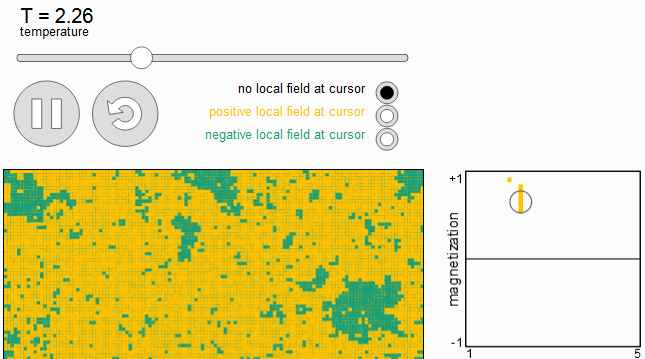
\includegraphics[width=\textwidth]{tLtTc}
	\end{subfigure}
	\;\;\;\;
	\begin{subfigure}[t]{0.45\textwidth}
		\caption{$T>T_c$}\label{fig:tGtTc}
		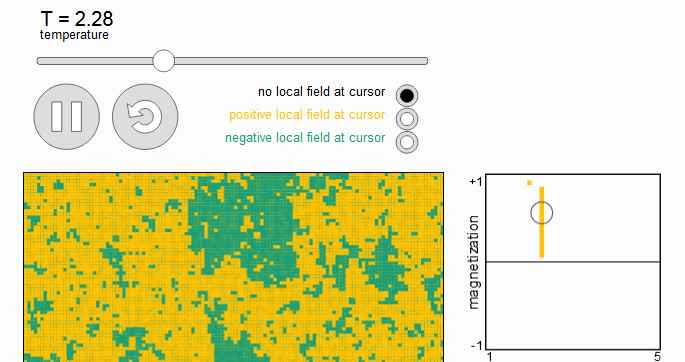
\includegraphics[width=\textwidth]{tGtTc}
	\end{subfigure}
\end{figure}

\begin{table}[H]
	\begin{center}
		\caption{Ising Model $T_c$}\label{eq:ising}
		\begin{tabular}{|l|c|c|}\hline
			$T$&M&$T_C$\\ \hline
			2&$\uparrow$&\\ \hline
			3&-&$[2,3]$\\ \hline
			2.5&-&$[2,2.5]$\\ \hline
			2.25&$\uparrow$&$[2.25,2.5]$\\ \hline
			2.32&-&$[2.25,2.32]$\\ \hline
			2.28&-&$[2.25,2.28]$\\ \hline
			2.26&$\uparrow$&$[2.26,2.28]$\\ \hline
			2.27&-&$[2.26,2.27]$\\ \hline
		\end{tabular}
	\end{center}
\end{table}

\begin{figure}[H]
	\caption{Correlation close to $R=T_c$}\label{fig:correlation1}
	\begin{subfigure}[t]{0.24\textwidth}
		\caption{$T=2.27$}
		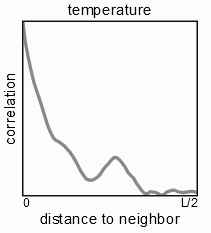
\includegraphics[width=\textwidth]{ising-correlation1}
	\end{subfigure}
	\begin{subfigure}[t]{0.24\textwidth}
		\caption{$T=2.27$}
		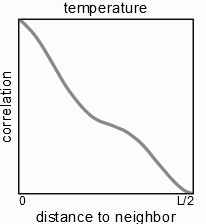
\includegraphics[width=\textwidth]{ising-correlation2}
	\end{subfigure}
	\begin{subfigure}[t]{0.24\textwidth}
		\caption{$T=2.27$}
		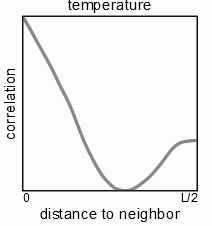
\includegraphics[width=\textwidth]{ising-correlation3}
	\end{subfigure}
	\begin{subfigure}[t]{0.24\textwidth}
		\caption{$T=2.27$}
		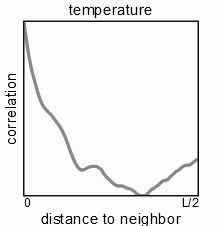
\includegraphics[width=\textwidth]{ising-correlation4}
	\end{subfigure}
\end{figure}

\begin{figure}[H]
	\caption{Correlation  $R<T_c$}\label{fig:correlation2}
	\begin{subfigure}[t]{0.24\textwidth}
		\caption{$T=2.20$}
		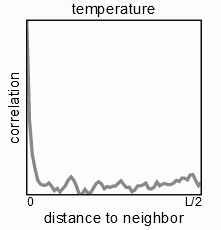
\includegraphics[width=\textwidth]{ising-correlation-20}
	\end{subfigure}
	\begin{subfigure}[t]{0.24\textwidth}
		\caption{$T=2.21$}
		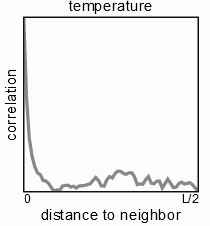
\includegraphics[width=\textwidth]{ising-correlation-21}
	\end{subfigure}
	\begin{subfigure}[t]{0.24\textwidth}
		\caption{$T=2.22$}
		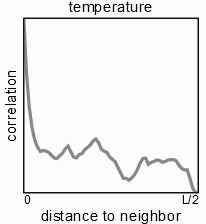
\includegraphics[width=\textwidth]{ising-correlation-22}
	\end{subfigure}
	\begin{subfigure}[t]{0.24\textwidth}
		\caption{$T=2.26$}
		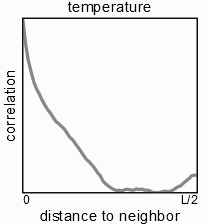
\includegraphics[width=\textwidth]{ising-correlation-26}
	\end{subfigure}
\end{figure}

\begin{table}[H]
	\begin{center}
		\caption{Percolation Model Interactive}\label{eq:percolation}
		\begin{tabular}{|c|c|}\hline
			&\\ \hline
		\end{tabular}
	\end{center}
\end{table}

\section{Landscapes, Clustering, Freezing and Hardness}

Based on the plot below--Figure \ref{fig:content_SATalpha}--showing percent satisfiability (SAT) relative to $\alpha$ for two different N:

\begin{enumerate}
	\item  Generally speaking, what happens in the solvability space of SAT problems?

	\item  What does the vertical red dashed line indicate?

	\item   Where do you expect the computational time would be largest along the $\alpha$ axis?

	\item   Is the SAT party problem above satisfiable?
	
	\begin{align*}
		p =& \text{Invite Priyanka}\\
		e =& \text {Invite Esatban}\\
		x =& \text{Invite Xiaojie. Then the constraints are:}\\
		p \lor& \bar{e} \text{: Chris} \numberthis \label{eq:chris}\\
		e \lor& x \text{: John} \numberthis \label{eq:john}\\
		\bar{x} \lor& \bar{p} \text{: Isa} \numberthis \label{eq:isa}
	\end{align*}
	Suppose $p$ is true($p=\top$). Then (\ref{eq:chris}) is satisfied, and (\ref{eq:isa}) yields:
	\begin{align*}
		\bar{x}=\top& \text{, so}\\
		x =& \bot \text{. and (\ref{eq:john}) is satisfied iff:}\\
		e =& \top 
	\end{align*}
	Hence we have a solution that satisfies (\ref{eq:chris}-\ref{eq:isa}): invite Priyanka only.
\end{enumerate}


\begin{figure}[H]
	\begin{center}
		\caption{percent satisfiability (SAT) relative to $\alpha$ for two different N}\label{fig:content_SATalpha}
		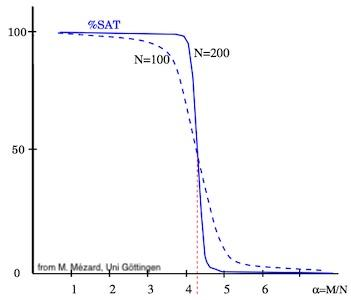
\includegraphics[width=0.6\textwidth]{content_SATalpha}
	\end{center}
\end{figure}
% bibliography go here

\bibliographystyle{unsrt}
\raggedright
\addcontentsline{toc}{section}{Bibliography}
\bibliography{computations}

\end{document}
